
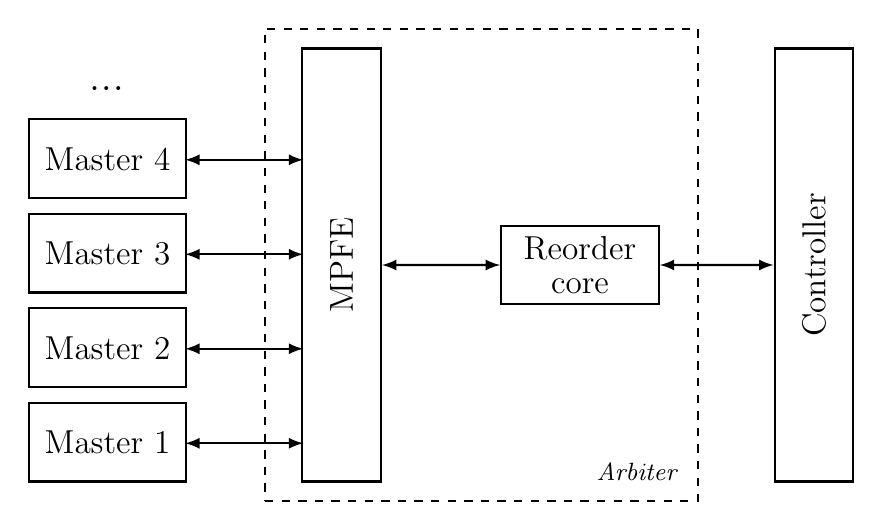
\begin{tikzpicture}[font={\fontsize{12pt}{12}\selectfont}]
    
\node[rectangle, draw, color=black, thick, anchor=south west, minimum width=2cm, minimum height=1cm, inner sep=0pt] (master1) at (0,0) {Master 1};
\node[rectangle, draw, color=black, thick, anchor=south west, minimum width=2cm, minimum height=1cm, inner sep=0pt] (master2) at (0,1.2) {Master 2};
\node[rectangle, draw, color=black, thick, anchor=south west, minimum width=2cm, minimum height=1cm, inner sep=0pt] (master3) at (0,2.4) {Master 3};
\node[rectangle, draw, color=black, thick, anchor=south west, minimum width=2cm, minimum height=1cm, inner sep=0pt] (master4) at (0,3.6) {Master 4};

\node[rectangle, draw, color=black, thick, anchor=south west, minimum width=5.5cm, minimum height=1cm, inner sep=0pt, rotate=90] (MPFE) at (4.5,0) {MPFE};

    \node at (1,5) {{\LARGE ...}};


\draw[<->, >=latex, thick] (2,0.5) -- (3.5,0.5) ;
\draw[<->, >=latex, thick] (2,1.7) -- (3.5,1.7) ;
\draw[<->, >=latex, thick] (2,2.9) -- (3.5,2.9) ;
\draw[<->, >=latex, thick] (2,4.1) -- (3.5,4.1) ;

\node[rectangle, draw, color=black, thick, anchor=south west, minimum width=2cm, minimum height=1cm, inner sep=0pt, align=center] (reorder) at (6,2.25) {Reorder\\ core};

\draw[<->, >=latex, thick] (MPFE.south) -- (reorder.west) ;

\node[rectangle, draw, color=black, thick, anchor=south west, minimum width=5.5cm, minimum height=1cm, inner sep=0pt, rotate=90] (controller) at (10.5,0) {Controller};

\draw[<->, >=latex, thick] (reorder.east) -- (controller.north) ;

\node[rectangle, draw, color=black, thick, anchor=south west, minimum width=5.5cm, minimum height=6cm, inner sep=0pt, dashed]  at (3,-0.25) {};

\node[anchor=south west] at (7.1,-0.1) {\textit{\small Arbiter}};

\end{tikzpicture}
